%%%%%%
%%%%%%%%%%%%%%%%%%%%%%%%
%
% $Author: Adhiraj Walse $
% $Datum: 2023-10-31  $
%$Pfad:Users/Documents/ML23-06-Magic-Wand-with-an-Arduino-Nano-33-BLE-sense/report/Contents/en/HardwareDescription.tex $
% $Version: 1.0 $
%
% $Short Description: Describe hardware that we use in our Magic Wand Project and testing on the hardware$
%%%%%%%%%%%%%%%%%%%%%%%%


\chapter{Hardware Description}
\label{chapter 3}

\section{Board Arduino Nano 33 BLE Sense}

The Arduino Nano 33 BLE Sense board serves as a prime example of edge computing. It integrates multiple sensors alongside BLE connectivity and wireless communication features \cite{Raj:2019}, making it suitable for a wide range of IoT and wearable applications. Equipped with sensors for temperature, pressure, magnetometry, acceleration, and gyroscopic measurements \cite{Raj:2019}, the board also includes a microphone and a proximity sensor. Its built-in BLE capabilities enable seamless interaction with other BLE-compatible devices, such as smartphones, facilitating remote data collection and control \cite{Bagur:2023}. At Magic Wand, our focus lies in leveraging the Accelerometer, Gyroscope, and Magnetometer sensors. The Arduino Nano 33 BLE Sense stands out as a versatile board, ideal for applications requiring sensor integration and wireless communication in IoT and wearable technologies \cite{Raj:2019}.

The Arduino Nano 33 BLE Sense is a compact, microcontroller-based development board designed to operate at a maximum of 3.3V. It is essential to avoid exceeding this voltage on its digital and analog pins \cite{Arduino:2021}. The board features a Bluetooth Low Energy (BLE) module, making it suitable for IoT applications \cite{Bagur:2023}. Powered by an nRF52840 processor, it boasts a 64 MHz clock speed, 256 KB of SRAM, and 1 MB of flash memory. Additionally, it includes 14 digital I/O pins, eight of which are analog input pins for connecting external components and sensors. The board’s power consumption is remarkably low, drawing only 10 mA per I/O pin \cite{Arduino:2021}.  

The Arduino Nano 33 BLE Sense supports high-level programming languages similar to C/C++ \cite{Emeritus:2023}. Programming for microcontrollers, including Arduino, is done on a host computer. Code is written and compiled using Arduino’s Integrated Development Environment (IDE) before being uploaded to the microcontroller for execution. To connect the board, a micro-USB cable is used, linking the board to a laptop. Once powered, a green LED next to the micro-USB port indicates a successful connection.

Additionally, Arduino offers several versions of the Nano 33 BLE board. This includes the Nano 33 BLE Sense and Nano 33 BLE Sense Lite. The Lite version lacks the HTS221 temperature and humidity sensor, instead featuring the LPS22HB pressure sensor, which can measure temperature but not humidity \cite{Arduino:2022}. Since our project focuses on the IMU sensor for gesture recognition, both versions are suitable for use. The following descriptions and hardware tests are based primarily on the Arduino Nano 33 BLE Sense.

\begin{figure}[h!]
	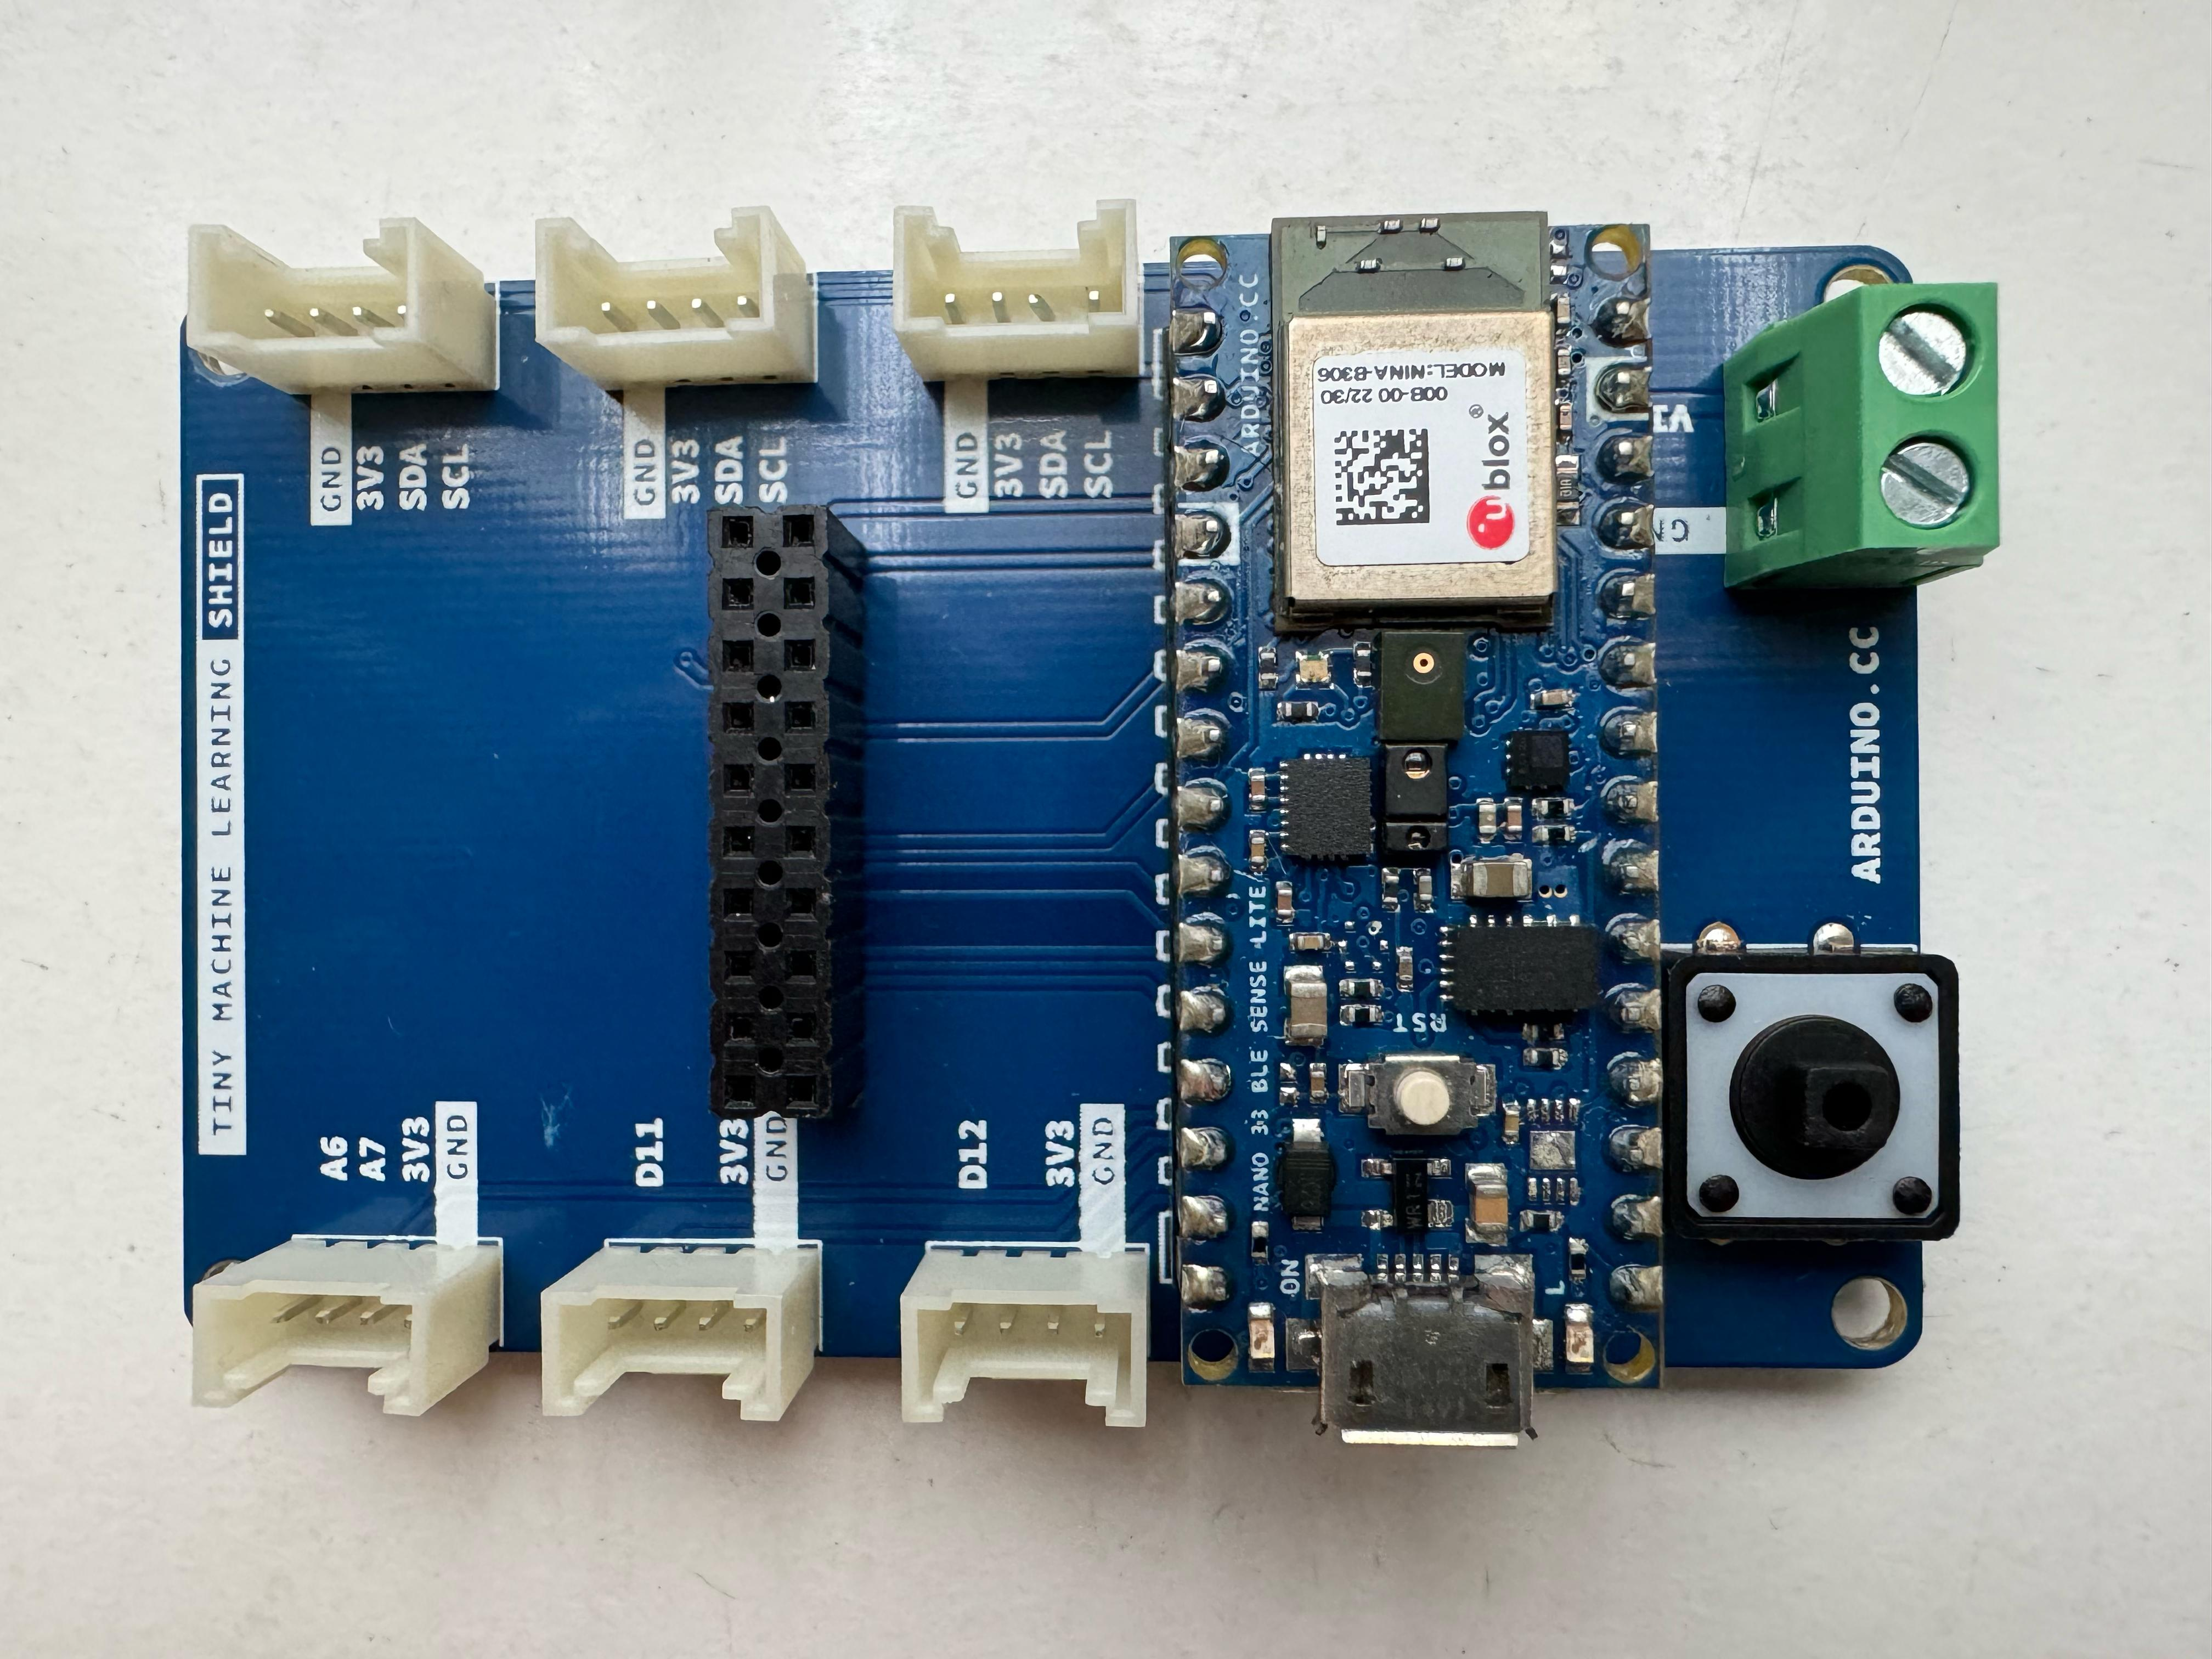
\includegraphics[width=\linewidth]{Images/HardwareDescription/ArduinoTop}
	\caption{\textbf{Top View of Board Arduino Nano 33 BLE Sense}}
	\label{fig:Top View of Board Arduino Nano 33 BLE Sense}
	\cite{Arduino:2023}
\end{figure}

\begin{figure}[h!]
	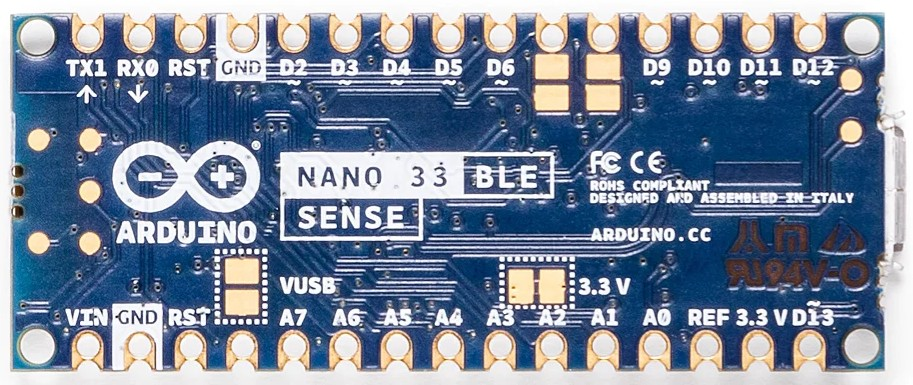
\includegraphics[width=\linewidth]{Images/HardwareDescription/ArduinoBottom}
	\caption{\textbf{Bottom View of Board Arduino Nano 33 BLE Sense}}
	\label{fig:Bottom View of Board Arduino Nano 33 BLE Sense} \cite{Arduino:2023}
\end{figure}


\section{Interfaces}

\subsection{Board Arduino Nano 33 BLE Sense: Components Overview}\label{BoardDescription}



The Arduino Nano 33 BLE Sense is equipped with several embedded sensors, including humidity, temperature, barometric pressure, proximity, and a microphone. These built-in components allow the board to be utilized for various practical applications without the need for additional circuitry \cite{Arduino:2021}. It supports standard communication protocols such as UART, I2C, and SPI, enabling seamless interaction with external circuits and sensors for data exchange. The board includes a micro-USB port for connecting to a laptop or desktop, which serves as both a power supply and a medium for file or data transfer via serial communication. While operating the board, it is crucial to ensure that no more than 3.3V is applied to its pins, as exceeding this voltage can result in permanent damage \cite{Arduino:2021}.

Below is a detailed description of each sensor embedded on the board:

\begin{center}
	\begin{tikzpicture}
		\ArduinoNanoTikz
		
		\node(HTS) at (-10,5){\textcolor{red}{\tiny HTS221}};
		\draw[line width=1pt,red]  (-6.3,2.8) -- (-10,4.9);
		\node(APD) at (-6,5){\textcolor{red}{\tiny APDS9960}};
		\draw[line width=1pt,red]  (-5,2.25) -- (-6,4.9);
		\node(LSM9DS1) at (-2,5){\textcolor{red}{\tiny LSM9DS1}};
		\draw[line width=1pt,red]  (-5,3.15) -- (-2,4.9);
		
		\node(LSM9DS1) at (1,5){\textcolor{red}{\tiny RGB Programmable LED}};
		\draw[line width=1pt,red]  (-3.6,2.95) -- (1,4.9);
		
		\node(HTS) at (1.5,2.25){\textcolor{red}{\tiny Nordic nRF 52840}};
		\draw[line width=1pt,red]  (-2,2.25) -- (0.5,2.25);
		
		\node(MP) at (-2,-0.75){\textcolor{red}{\tiny MP34DT05-A}};
		\draw[line width=1pt,red]  (-3.9,2.25) -- (-1.75,-0.6);
		
		\node(MP) at (-6,-0.75){\textcolor{red}{\tiny LPS22HB}};
		\draw[line width=1pt,red]  (-4.5,1.0) -- (-6,-0.6);
		
		\node(LEDPower) at (-11.5,3.55){\textcolor{red}{\tiny Power LED}};
		\draw[line width=1pt,red]  (-10.8,3.55) -- (-10,3.55);
		
		\node(USB) at (-12,2.25){\textcolor{red}{\tiny Micro-USB Port}};
		\draw[line width=1pt,red]  (-11.1,2.25) -- (-10.2,2.25);
		
		\node(LEDOrange) at (-11.8,0.8){\textcolor{red}{\tiny Progammable LED}};
		\draw[line width=1pt,red]  (-10.8,0.8) -- (-10,0.8);
		
	\end{tikzpicture}
	\captionof{figure}{}\label{ArduinoNano33BLESenseArchitecture}
\end{center}

\begin{itemize}
	\item LSM9DS1 - \ac{imu} features a 3D accelerometer, gyroscope and magnetometer and allows you to detect orientation, motion or vibrations in your project \cite{Alushi:2023}.
	\item  APDS-9960 - The APDS-9960 chip allows for measuring digital proximity and ambient light as well as for detecting RGB colors and gestures \cite{Avago:2015}.
	\item  LPS22HB - The LPS22HB picks up on barometric pressure and allows for a 24-bit pressure data output between 260 and 1260 hPa. This data can also be processed to calculate the height above sea level of the current location \cite{Stm:2017}.
	\item HTS221 - The HTS221 capacitive digital sensor measures relative humidity and temperature. It has a temperature accuracy of ± 0.5 °C (between 15-40 °C) and is perfectly suited to detect ambient temperature \cite{Stm:2023}.
	\item MP34DT05 - The MP34DT05 microphone allows you to capture and analyze sound in real-time and can be used to create a voice interface for your project\cite{Stm:2021}.
	\item USB port - USB port allows you to connect Arduino Nano 33 BLE sense to your machine.
	\item LEDs - There are 3 different LEDs that can be accessed on the Nano BLE Sense: \ac{rgb}(Programmable LED), the built-in LED(Programmable LED) and the power LED
\end{itemize}

\subsubsection{LEDs function in Board Arduino Nano 33 BLE Sense}
Apart from the Power LED indicate the board is powered, there are two LEDs in the board: Programmable LED(orange) and the RGB Programmable LED. The orange LED sparkles when it is connected to the computer. The RGB LED can be used during the creation of the actions that we perform. For example, in our project, each gesture can use one color to represent a specific gesture, indicating as the recognizing function. 

\section{Arduino Nano 33 BLE Pin Configuration}

The \textbf{Arduino Nano 33 BLE} is an advanced version of the Arduino Nano board that is based on a powerful processor, the nRF52840. The following is the pin configuration of the board:

\subsection{Pin Configuration}
\textbf{Digital Pins:}
\begin{itemize}[noitemsep]
	\item The board has \textbf{14 digital I/O pins} that receive only two values: HIGH or LOW.
	\item These pins can function as input or output based on the requirement.
	\item When the pins receive 5V, they are in a HIGH state; when they receive 0V, they are in a LOW state.
\end{itemize}

\textbf{Analog Pins:}
\begin{itemize}[noitemsep]
	\item The board has a total of \textbf{8 analog pins} (A0–A7).
	\item These pins measure analog voltage ranging between 0 to 5V and can get any value as opposed to digital pins, which only receive HIGH or LOW values.
\end{itemize}

\textbf{PWM Pins:}
\begin{itemize}[noitemsep]
	\item All digital pins can be used as PWM pins.
	\item These pins generate analog results using digital means.
\end{itemize}

\textbf{SPI Pins:}
\begin{itemize}[noitemsep]
	\item The board supports the \textbf{Serial Peripheral Interface (SPI)} communication protocol.
	\item SPI is used to communicate between the controller and peripheral devices such as shift registers and sensors.
	\item Two pins, \textbf{MISO} (Master Input Slave Output) and \textbf{MOSI} (Master Output Slave Input), are used for SPI communication.
\end{itemize}

\textbf{I2C Pins:}
\begin{itemize}[noitemsep]
	\item The board supports the \textbf{I2C communication protocol}, a two-wire protocol.
	\item It includes two pins: \textbf{SDL} and \textbf{SCL}.
\end{itemize}

\textbf{UART Pins:}
\begin{itemize}[noitemsep]
	\item The board features the \textbf{UART communication protocol} for serial communication.
	\item It includes two pins: \textbf{Rx} (receiving pin) and \textbf{Tx} (transmitting pin).
\end{itemize}

\textbf{External Interrupts Pins:}
\begin{itemize}[noitemsep]
	\item All digital pins can be used as external interrupt pins.
	\item This feature allows the main running program to be interrupted and handle emergency instructions.
\end{itemize}

\textbf{LED at Pin 13 and AREF Pin:}
\begin{itemize}[noitemsep]
	\item There is an \textbf{LED connected to pin 13} of the board.
	\item The \textbf{AREF pin} is used as a reference voltage for input voltage.
\end{itemize}

\begin{figure}[h!]
	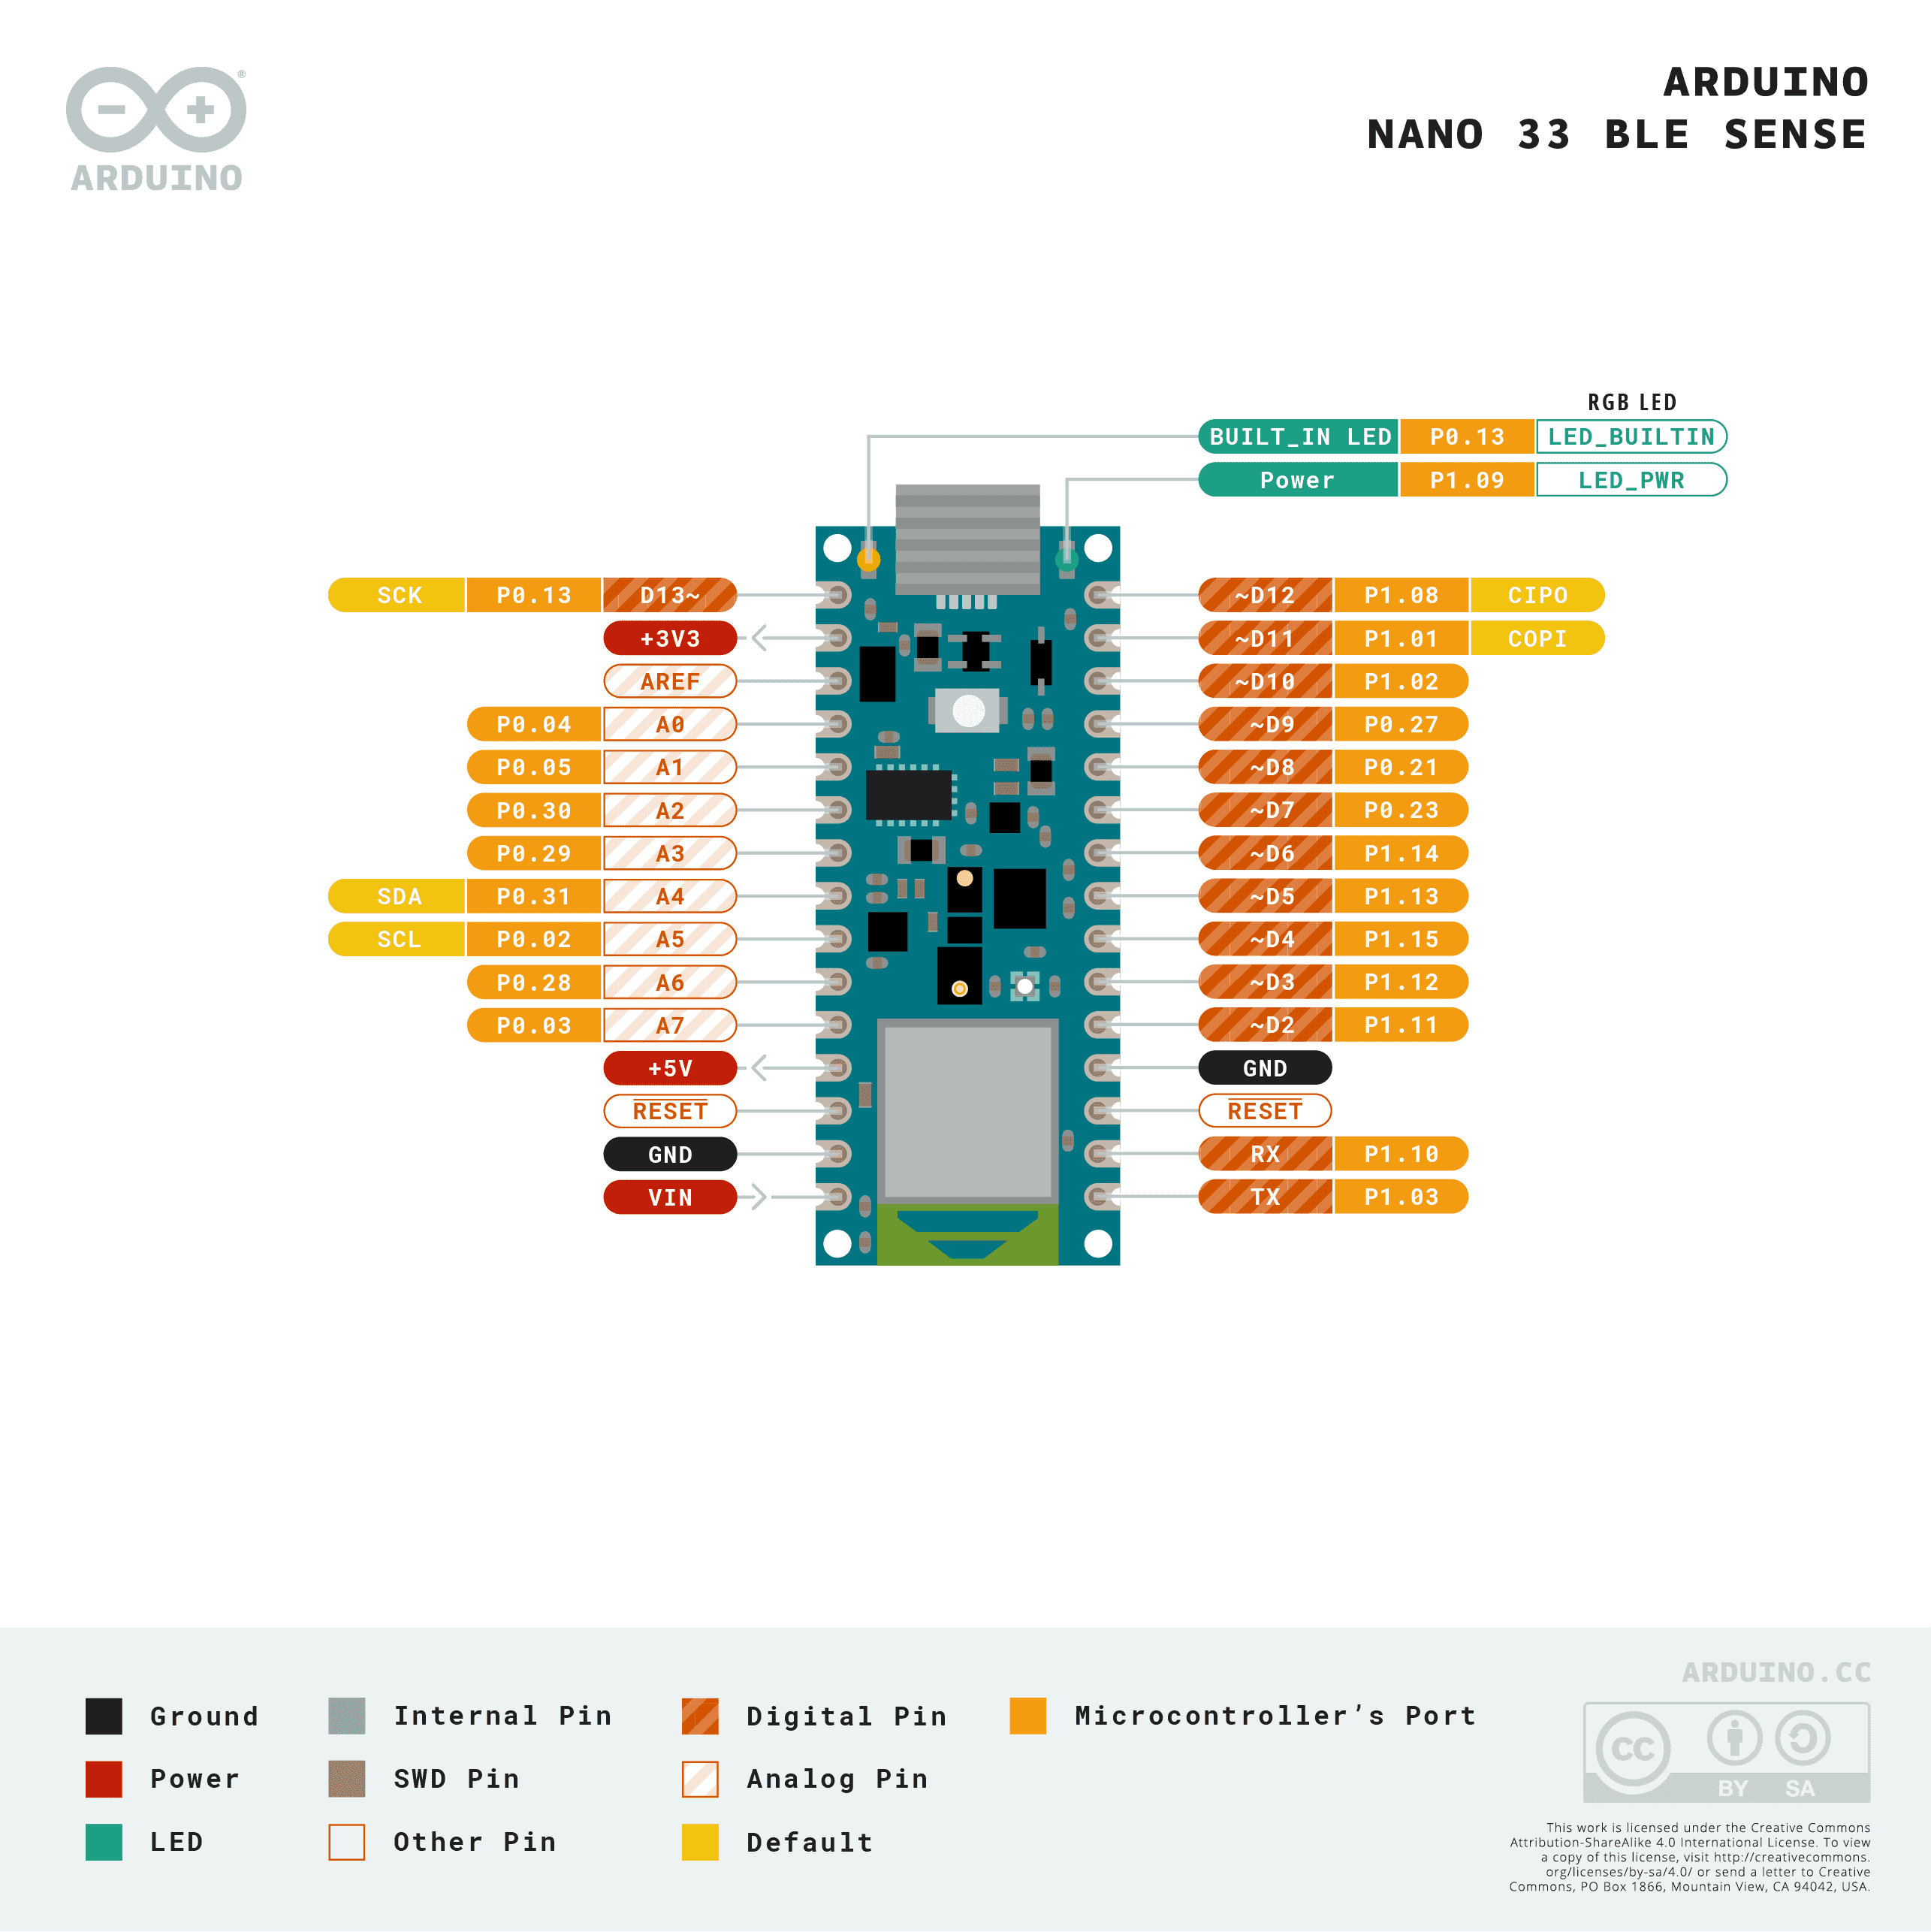
\includegraphics[width=\linewidth]{Images/HardwareDescription/Pin_Configuration}
	\caption{\textbf{Arduino Nano 33 BLE Pin Configuration}}
	\label{Arduino Nano 33 BLE Pin Configuration} \cite{Arduino:2023}
\end{figure}

\section{Data Quality in Hardware Description}

In the hardware description of our Magic Wand project with Arduino Nano 33 BLE Sense, we consider the following aspects related to data quality:

\begin{enumerate}
	\item \textbf{Sensor Accuracy:} The sensors embedded in the Arduino Nano 33 BLE Sense board deliver precise measurements of environmental parameters such as motion, orientation, temperature, humidity, and pressure \cite{Dhow:2024}.
	
	\item \textbf{Resolution:} Each sensor has a defined resolution, representing the smallest detectable input change. For instance, the accelerometer’s resolution is \textless{}insert value\textgreater{}, allowing detection of subtle motion variations.
	
	\item \textbf{Sampling Rate:}The board supports high sampling rates, enabling real-time data acquisition at \textless{}insert frequency\textgreater{} Hz. This is essential for applications requiring continuous and responsive data collection.
	
	\item \textbf{Noise Level:} Sensor data may exhibit noise due to factors such as environmental conditions, sensor imperfections, or electromagnetic interference. The board minimizes noise using calibration and filtering techniques, ensuring high data fidelity.
	
	\item \textbf{Calibration:} Calibration processes are applied to enhance the accuracy and reliability of sensor readings. These procedures involve fine-tuning sensor settings and using correction factors to address systematic errors \cite{Edm:2015}.
	
	\item \textbf{Data Transmission:} Sensor data is transmitted from the Arduino Nano 33 BLE Sense board to other devices using wireless communication protocols such as Bluetooth Low Energy (BLE). Data transmission is efficient, ensuring minimal latency and reliable delivery.
	
	\item \textbf{Data Integrity:} To maintain data integrity during transmission and processing, error detection and correction mechanisms are implemented. These measures help identify and resolve issues like data loss or corruption \cite{TensorFlow:2023}.
	
	\item \textbf{Power Consumption:} The Arduino Nano 33 BLE Sense is designed for low power consumption, making it ideal for battery-powered applications. Its optimized power management extends battery life without compromising continuous data collection.
\end{enumerate}

By addressing these aspects of data quality in the hardware description, we ensure the reliability and accuracy of sensor data used in our Magic Wand project.
\begin{center}
	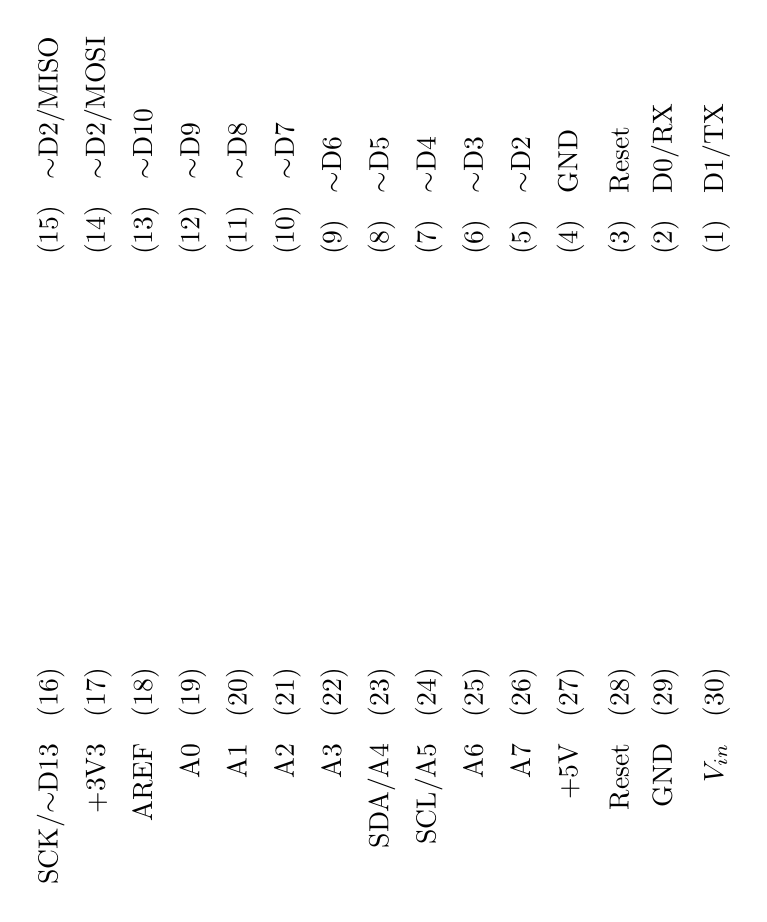
\begin{tikzpicture}
		
		\ArduinoNanoTikz
		
		\node[rotate=90,right] (Pin1) at (-0.91,4.6) {(1) \; D1/TX};
		\node[rotate=90,right] (Pin2) at (-1.56,4.6) {(2) \; D0/RX};
		\node[rotate=90,right] (Pin3) at (-2.11,4.6) {(3) \; Reset};
		\node[rotate=90,right] (Pin4) at (-2.76,4.6) {(4) \; GND};
		\node[rotate=90,right] (Pin5) at (-3.36,4.6) {(5) \; $\sim$D2};
		\node[rotate=90,right] (Pin6) at (-3.96,4.6) {(6) \; $\sim$D3};
		\node[rotate=90,right] (Pin7) at (-4.56,4.6) {(7) \; $\sim$D4};
		\node[rotate=90,right] (Pin8) at (-5.16,4.6) {(8) \; $\sim$D5};
		\node[rotate=90,right] (Pin9) at (-5.76,4.6) {(9) \; $\sim$D6};
		\node[rotate=90,right] (Pin10) at (-6.36,4.6) {(10) \; $\sim$D7};
		\node[rotate=90,right] (Pin11) at (-6.96,4.6) {(11) \; $\sim$D8};
		\node[rotate=90,right] (Pin12) at (-7.56,4.6) {(12) \; $\sim$D9};
		\node[rotate=90,right] (Pin13) at (-8.16,4.6) {(13) \; $\sim$D10};
		\node[rotate=90,right] (Pin14) at (-8.76,4.6) {(14) \; $\sim$D2/MOSI};
		\node[rotate=90,right] (Pin15) at (-9.36,4.6) {(15) \; $\sim$D2/MISO};
		
		
		\node[rotate=90,left] (Pin30) at (-0.91,-0.4) { $V_{in}$ \; (30)};
		\node[rotate=90,left] (Pin1) at (-1.56,-0.4) {GND \; (29)};
		\node[rotate=90,left] (Pin2) at (-2.11,-0.4) {Reset \; (28)};
		\node[rotate=90,left] (Pin3) at (-2.76,-0.4) {+5V \; (27)};
		\node[rotate=90,left] (Pin4) at (-3.36,-0.4) {A7 \; (26)};
		\node[rotate=90,left] (Pin5) at (-3.96,-0.4) {A6 \; (25)};
		\node[rotate=90,left] (Pin6) at (-4.56,-0.4) {SCL/A5 \; (24)};
		\node[rotate=90,left] (Pin7) at (-5.16,-0.4) {SDA/A4 \; (23)};
		\node[rotate=90,left] (Pin8) at (-5.76,-0.4) {A3 \; (22)};
		\node[rotate=90,left] (Pin9) at (-6.36,-0.4) {A2 \; (21)};
		\node[rotate=90,left] (Pin10) at (-6.96,-0.4) {A1 \; (20)};
		\node[rotate=90,left] (Pin11) at (-7.56,-0.4) {A0 \; (19)};
		\node[rotate=90,left] (Pin12) at (-8.16,-0.4) {AREF \; (18)};
		\node[rotate=90,left] (Pin13) at (-8.76,-0.4) {+3V3 \; (17)};
		\node[rotate=90,left] (Pin14) at (-9.36,-0.4) {SCK/$\sim$D13 \; (16)};
		
	\end{tikzpicture}
	\captionof{figure}[Pin assignment of the Arduino Nano 33 BLE Sense]{Pin assignment of the Arduino Nano 33 BLE Sense; note that the orange built-in LED is connected to pin D13 and the power LED to pin D1. The built-in RGB LED occupies pins D18, D19 and D20.}
\end{center}

\subsection{Specifications of Arduino Nano 33 BLE Sense}


\subsubsection*{NINA B306 Module}
\begin{enumerate}[label=\arabic*.]
	\item Processor:
	\begin{itemize}[label=-]
		\item 64 MHz Arm® Cortex-M4F (with FPU)
		\item 1 MB Flash + 256 KB RAM
	\end{itemize}
	\item Bluetooth® 5 multiprotocol radio:
	\begin{itemize}[label=-]
		\item 2 Mbps
		\item +8 dBm TX power
		\item -95 dBm sensitivity
		\item 4.8 mA in TX (0 dBm)
		\item 4.6 mA in RX (1 Mbps)
		\item Integrated balun with 50 Ohm single-ended output
		\item IEEE 802.15.4 radio support
	\end{itemize}
	\item Peripherals:
	\begin{itemize}[label=-]
		\item 12 Mbps USB
		\item NFC-A tag
		\item Arm CryptoCell CC310 security subsystem
		\item QSPI/SPI/TWI/I2S/PDM/QDEC
		\item 32 MHz SPI
		\item Quad SPI interface 32 MHz
		\item 12-bit 200 ksps ADC
		\item 128 bit AES/ECB/CCM/AAR co-processor
	\end{itemize}
\end{enumerate}

\subsubsection*{LSM9DS1 (9 axis IMU)}\cite{Warden:2020}
\begin{enumerate}[label=\arabic*.]
	\item 3 acceleration channels, 3 angular rate channels, 3 magnetic field channels
	\item $\pm$2/$\pm$4/$\pm$8/$\pm$16 g linear acceleration full scale
	\item $\pm$4/$\pm$8/$\pm$12/$\pm$16 gauss magnetic full scale
	\item $\pm$245/$\pm$500/$\pm$2000 dps angular rate full scale
	\item 16-bit data output
\end{enumerate}




\section{Data quantity in Hardware Description}

\begin{enumerate}
	\item \textbf{Sensor Data}: The Arduino Nano 33 BLE Sense board is equipped with a variety of sensors, including an accelerometer, a gyroscope, and a magnetometer. These sensors generate a large amount of data as you wave the magic wand. For instance, in one experiment, a window size of 2 seconds was used, which means 200 rows of accelerometer data or 600 values of x, y, and z acceleration axis were fed into the model. \cite{Miller:2022}
	
	\item \textbf{Data Processing Capacity}: The Arduino Nano 33 BLE Sense board has a 32-bit ARM Cortex-M4 CPU running at 64 MHz, which allows it to process a significant amount of sensor data in real-time.
	
	\item \textbf{Memory}: The board has 1MB of flash memory and 256KB of SRAM. This memory is used to store the program code and handle runtime operations, including storing sensor data and machine learning model parameters.
	
	\item \textbf{Machine Learning Model}: The size of the machine learning model used in the project also affects the quantity of data. The model needs to be small enough to fit into the board's memory along with the program code.
	
	\item \textbf{Data Transmission}: The board also has a built-in Bluetooth Low Energy module, which can be used to transmit sensor data to another device for further processing. \cite{TensorFlow:2023}
	
\end{enumerate}


\section{Constraints}
\subsubsection{Arduino Nano 33 BLE Sense}
\begin{itemize}[label=--]
	\item Operating Voltage: 3.3V
	\item Power Consumption:
	\begin{itemize}[label=--,leftmargin=*]
		\item Maximum 15mA in low power mode
		\item Maximum 60mA in active mode
	\end{itemize}
	\item Operating Temperature Range: -40°C to 85°C
	\item Memory Constraints: 1 MB Flash + 256 KB RAM
	\item Communication Interfaces: USB, Bluetooth 5, NFC-A, SPI, I2C, QSPI, etc.\cite{Arduino:2015}
\end{itemize}

\subsubsection*{Sensors}
\begin{itemize}[label=--]
	\item Accelerometer:
	\begin{itemize}[label=--,leftmargin=*]
		\item Measurement Range: ±8g
		\item Operating Temperature Range: -40°C to 85°C
	\end{itemize}
	\item Gyroscope:
	\begin{itemize}[label=--,leftmargin=*]
		\item Measurement Range: ±2000 dps
		\item Operating Temperature Range: -40°C to 85°C \cite{Arduino:2021}
	\end{itemize}
	
\end{itemize}


\subsubsection*{Actuators}
\begin{itemize}[label=--]
	\item RGB LEDs:
	\begin{itemize}[label=--,leftmargin=*]
		\item Power Requirements: Voltage, Current
		\item Operating Temperature Range
	\end{itemize}
	\item Buzzer/Speaker:
	\begin{itemize}[label=--,leftmargin=*]
		\item  Voltage, Current, Sound Output Levels
	\end{itemize}
	
\end{itemize}

\subsubsection*{Power Supply}
\begin{itemize}[label=--]
	\item Input Voltage Range: Specify the acceptable input voltage range.
	\item Power Consumption: Estimate the overall power consumption of the system.
\end{itemize}

\subsubsection*{Physical Constraints}
\begin{itemize}[label=--]
	\item Size and Dimensions: Ensure compatibility with the project enclosure or housing.
	\item Mounting Requirements: Specify any specific mounting requirements for the components.
\end{itemize}

\subsubsection*{Environmental Constraints}
\begin{itemize}[label=--]
	\item Environmental Protection: Ensure components are suitable for the intended environmental conditions (e.g., moisture resistance, dust resistance).
	\item Operating Conditions: Specify any limitations or special considerations for operating in certain environments.\cite{Arduino:2021}
\end{itemize}



\section{Dimensions of the Arduino Nano 33 BLE Sense}



The Arduino Nano 33 BLE Sense is a highly compact development board, measuring just 45mm x 18mm. Its small form factor makes it particularly well-suited for wearable devices and other space-constrained applications. Despite its size, the board is equipped with a wide range of sensors and features, offering versatility for various projects.

It is important to note that these dimensions apply to the board without headers. If you are using a version with pre-soldered headers or attaching additional components, the overall dimensions of your hardware setup may change. For precise measurements, always consult the specifications of your specific board and components \cite{Arduino:2023}.


\section{Sensor Accelerometer, Gyroscope, and Magnetometer LSM9DS1}\label{boardsensor}

Magic Wand gesture detection is mainly based on the sensor LSM9DS1 at the board. It is a system-in-package featuring a 3D digital linear acceleration sensor, a 3D digital angular rate sensor, and a 3D digital magnetic sensor. A tiny device called an Inertial Measurement Unit (IMU) in the sensor is used to detect the motions physically \cite{Alushi:2023}. It has several components, including magnetometer, gyroscope, and accelerometer. By monitoring  acceleration and angular velocity changes, the IMU sensor is critical for identifying an object's orientation and movement in real-time \cite{Alushi:2023}.





\subsection*{Example Code for Arduino Nano 33 BLE Sense}
Below is a simple example demonstrating how to use the built-in microphone on the Arduino Nano 33 BLE Sense:

\begin{code}
	\begin{Arduino}
		// Include the PDM library
		#include <PDM.h>
		
		// Buffer to store the microphone data
		short sampleBuffer[256];
		
		// Variable to store the sound level
		int soundLevel = 0;
		
		// Callback function for PDM data
		void onPDMdata() {
			// Read the PDM data
			int bytesAvailable = PDM.available();
			PDM.read(sampleBuffer, bytesAvailable);
			
			// Calculate the sound level
			soundLevel = 0;
			for (int i = 0; i < bytesAvailable / 2; i++) {
				soundLevel += abs(sampleBuffer[i]);
			}
			soundLevel /= bytesAvailable / 2;
		}
		
		void setup() {
			// Initialize serial communication
			Serial.begin(9600);
			while (!Serial);
			
			// Initialize PDM with a sample rate of 16 kHz and 16-bit resolution
			PDM.begin(1, 16000);
			PDM.onReceive(onPDMdata);
		}
		
		void loop() {
			// Print the sound level to the serial monitor
			Serial.println(soundLevel);
			delay(100);
		}
	\end{Arduino}
	\caption{Simple example using of the builtin microphone of the Arduino Nano 33 BLE Sense}\label{code:microphone}
\end{code}

\begin{code}
	\begin{Arduino}
		// Include the ArduinoBLE library
		#include <ArduinoBLE.h>
		
		// Create a BLE service
		BLEService batteryService("1101");
		
		// Create a BLE characteristic
		BLEUnsignedCharCharacteristic batteryLevelChar("2101", BLERead | BLENotify);
		
		void setup() {
			// Initialize serial communication
			Serial.begin(9600);
			while (!Serial);
			
			// Set up the built-in LED pin
			pinMode(LED_BUILTIN, OUTPUT);
			
			// Initialize BLE
			if (!BLE.begin()) {
				Serial.println("Starting BLE failed!");
				while (1);
			}
			
			// Set the BLE local name and advertised service
			BLE.setLocalName("BatteryMonitor");
			BLE.setAdvertisedService(batteryService);
			
			// Add characteristic to the service
			batteryService.addCharacteristic(batteryLevelChar);
			
			// Add the service and start advertising
			BLE.addService(batteryService);
			BLE.advertise();
			
			Serial.println("Bluetooth device active, waiting for connections...");
		}
		
		void loop() {
			// Wait for a BLE central to connect
			BLEDevice central = BLE.central();
			
			if (central) {
				Serial.print("Connected to central: ");
				Serial.println(central.address());
				
				// Turn on the built-in LED
				digitalWrite(LED_BUILTIN, HIGH);
				
				// Loop while the central device is connected
				while (central.connected()) {
					int battery = analogRead(A0);
					int batteryLevel = map(battery, 0, 1023, 0, 100);
					
					Serial.print("Battery Level is now: ");
					Serial.println(batteryLevel);
					
					// Update the characteristic value
					batteryLevelChar.writeValue(batteryLevel);
					
					delay(200);
				}
				
				// Turn off the built-in LED
				digitalWrite(LED_BUILTIN, LOW);
				Serial.print("Disconnected from central: ");
				Serial.println(central.address());
			}
		}
	\end{Arduino}
	\caption{Example of a BLE Battery Monitor using Arduino Nano 33 BLE Sense}\label{code:battery-monitor}
\end{code}

\pagebreak
\section{Inertial Measurement Unit (IMU)}\label{IMU}

\subsection{Description}
An Inertial Measurement Unit (IMU) is an electronic system that measures movement across multiple axes using three primary sensors: an accelerometer, a gyroscope, and a magnetometer.\cite{Qureshi:2017} These sensors work together to provide data on acceleration, rotational motion, and magnetic fields, making IMUs essential for a wide range of applications such as navigation, fitness tracking, and robotics.\cite{Qureshi:2017}

{General}
IMUs have become increasingly common in microcontroller projects, with some boards, such as the Arduino Nano 33 BLE Sense, featuring integrated IMUs for seamless development of motion-sensitive applications.\cite{Zhou:2020}

\subsection{Specific Sensors}
\textbf{Continuous Operation ("Always-On" Mode)}
The LSM9DS1 supports an "Always-On" mode, ensuring continuous operation even when the main system is in a low-power state.\cite{Zhou:2020} This is critical for uninterrupted motion monitoring in devices like the Magic Wand, where gestures must be tracked instantly. With a power consumption of just 0.55 mA in high-performance mode, it provides precise and reliable motion data while preserving battery life.\cite{Zhou:2020}

\textbf{Tilt Detection}
Using the accelerometer, the IMU can detect orientation changes with minimal power usage. Tilt detection is particularly useful for identifying subtle shifts in position, enhancing the responsiveness of gesture-based controls.\cite{Zhou:2020}

\textbf{Significant Motion Detection}
The accelerometer enables significant motion detection (SMD), which recognizes large-scale movements. SMD can be used to activate specific device functions, such as waking the system from sleep mode or triggering predefined actions based on significant gestures.\cite{Zhou:2020}

The LSM9DS1 is a versatile and energy-efficient IMU with advanced sensing capabilities, supporting a range of applications where motion detection, orientation tracking, and gesture recognition are essential. Its compact design, low power consumption, and robust environmental tolerance make it a reliable choice for portable, battery-powered devices like the Magic Wand.\cite{Zhou:2020}

An \ac{imu} consists of three sensors that measure an object's orientation, position, vibration and movement in 3D space in real-time. These sensors are typically arranged in a pattern, including a tri-axial accelerometer, gyroscope, and magnetometer\cite{Ahmad:2013}. An accelerometer is used to measure the change in velocity of a moving or vibrating object\cite{Ahmad:2013}. Gyroscope measures the angular rotation\cite{Ahmad:2013}. A Magnetometer is used to measure yaw angle rotation, calibrating to the gyroscope data to improve the big drift issue\cite{Ahmad:2013}. 

The accelerometer functions by gauging the acceleration (Ax, Ay, Az), which denotes the rate of acceleration change over time. The acceleration values along each axis are conventionally expressed in units of meters per second squared $(m/s^2)$ \cite{Vernier:2023}. To illustrate, if the LSM9DS1 records an acceleration of 15 $m/s^2$ along the x-axis, this signifies that the object under observation is experiencing a velocity increment of 15 meters per second every second in the x-direction.

A gyroscope, designed to quantify angular speed ($\omega$x, $\omega$y, $\omega$z), serves as an indicator of the object's orientation change rate along each axis. Angular velocity along each axis is commonly expressed in degrees per second ($\circ$/s) \cite{Zhuang:2020}. For instance, when the LSM9DS1 records an angular velocity of 100$\circ$/s along the z-axis, it signifies that the measured object is undergoing rotation at a rate of 100 degrees per second around the z-axis. Refer to the accompanying figure for visualization.

In the context of a magnetometer, the x, y, and z axes (Mx, My, Mz) typically delineate the three-dimensional space in which the magnetic field is being assessed. The x-axis typically corresponds to the horizontal component of the magnetic field, the y-axis signifies the vertical component, and the z-axis reflects the magnetic field strength \cite{Kostiainen:2023}. This three-dimensional measurement provides a comprehensive understanding of the magnetic field in the surrounding space.

\begin{figure}[h!]\centering
	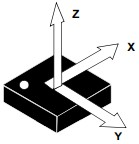
\includegraphics[width=6cm]{Images/HardwareDescription/AccelerometerForce}
	\caption{\textbf{Accelerometer Accerlerations Directions}}
	\label{fig:Acceleromter}
	\cite{Stm:2015}
\end{figure}

\begin{figure}[h!]\centering
	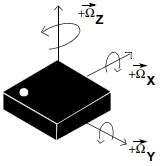
\includegraphics[width=6cm]{Images/HardwareDescription/AngularRotation}
	\caption{\textbf{Gyroscope Angular Directions}}
	\label{fig:Gyroscope}
	\cite{Stm:2015}
\end{figure}

\begin{figure}[h!]\centering
	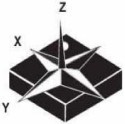
\includegraphics[width=6cm]{Images/HardwareDescription/MagnetometerDirection}
	\caption{\textbf{Magnetometer Directions}}
	\label{fig:Magnetometer}
	\cite{Stm:2015}
\end{figure}

IMUs can be classified into two main categories based on the type of sensors used: \ac{mems} IMUs and \ac{FOG} IMUs. MEMS IMUs use small mechanical sensors that are etched onto a silicon chip, while FOG IMUs use optical fibers to measure angular velocity. MEMS IMUs are typically smaller and less expensive but are also less accurate and have a shorter lifespan compared to FOG IMUs\cite{Deppe:2017}.

IMU is sent to a microcontroller or computer, and software is written to read the data from the sensors and perform the necessary calculations. There are also many libraries and software packages available that can simplify the process of working with IMUs.

IMUs are commonly used in a variety of applications, Industry Quality Control, Medical Rehabilitation, Robotics, Navigation Systems, Sports Learning and Augmented Reality Systems since they are essential to accurately measure the movement and orientation of the device for further function development \cite{Ahmad:2013}. In general, they are used for: 

\textbf{Orientation tracking:} IMUs can follow the orientation of an object in space by using a combination of acceleration and angular velocity sensors. The data from these sensors can be used to calculate the object's orientation. Robotics technology is one of the regions that require linear and angular data for the movements so robots can perform daily routines and advanced tasks similar to humans \cite{Ahmad:2013}.  

\textbf{Motion sensing:}  Detecting motion and acceleration changes is also one function that IMUs can achieve. Ryan et al. suggested integrating a miniaturized IMU sensor into the ball, comprising a tri-axial gyroscope and tri-axial accelerometer. Their initial experiment employed ball kinematics knowledge to estimate the drift error arising from measurements \cite{McGinnis:2011}. Subsequent research efforts enhanced data accuracy by cross-referencing the measurements with a high-speed motion analysis system consisting of 10 cameras (VICON) \cite{McGinnis:2012}.

\textbf{Navigation System:} IMUs are marked as an upgrade in the Global Positioning System (GPS) to navigate by combining data from the acceleration and angular velocity sensors with information for better data accuracy. Also, IMU can provide locations where no GPS signals are detected as an alternative option in the car and aircraft in case of emergency \cite{Ahmad:2013}. 

However, IMUs face a significant challenge due to the susceptibility of the underlying gyroscopes and accelerometers to measurement errors. This poses a fundamental issue for all IMUs as gyroscopes inherently exhibit drift, and accelerometers may introduce inaccuracies, resulting in misestimations of orientation concerning gravity. Despite incorporating minor measurement errors, the guidance system continually integrates the calculated position results with the original position information (refer to trajectory calculation). Although individual errors may be minor, their persistence across positions leads to cumulative effects known as "drift." Over time, this accumulation causes a widening disparity between the system's perceived and actual locations, and it becomes impossible to eliminate these errors \cite{Harris:2023}. Therefore, drift remains a fundamental challenge for any IMUs.
\subsection{Specifications}
\begin{itemize}
	\item 3 acceleration channels, 3 angular rate channels, 3 magnetic field channels.
	\item $\pm2/\pm4/\pm8/\pm16$ g linear acceleration full scale.
	\item $\pm4/\pm8/\pm12/\pm16$ gauss magnetic full scale.
	\item $\pm245/\pm500/\pm2000$ dps angular rate full scale.
	\item 16-bit data output.
\end{itemize}

3D digital linear acceleration sensor: Measures linear motion with a full scale of ±2g/±4g/±8g/±16g.\newline
3D digital angular rate sensor: Tracks rotational motion with an angular rate range of ±245/±500/±2000 degrees per second (dps).\newline
3D digital magnetic sensor: Detects magnetic fields with a full scale of ±4/±8/±12/±16 gauss.\newline
This compact and versatile IMU includes both I²C and SPI serial interfaces and supports a power-down mode for smart power management. It is available in a plastic land grid array (LGA) package and operates reliably across a wide temperature range from -40 °C to +85 °C.

\subsection{Libraries}

A library refers to a collection of pre-written code that can be used by developers to perform specific tasks or functions without having to write the code from scratch. Libraries are designed to make the development process easier and more efficient by providing pre-built solutions to common programming challenges.

\subsubsection{Wire.h}
\texttt{Wire.h} is a library in Arduino that allows for communication between I2C devices. I2C stands for Inter-Integrated Circuit, which is a synchronous serial communication protocol used for connecting microcontrollers to peripheral devices. \texttt{Wire.h} provides functions for initializing the I2C bus, sending and receiving data over the bus, and managing multiple devices on the same bus. With this library, developers can easily connect multiple I2C devices, such as sensors or displays, to an Arduino board \cite{Ardc; Ari21}.

\subsubsection{Kalman.h}
\texttt{Kalman.h} is a library that implements the Kalman filter algorithm. The Kalman filter is a mathematical technique used to estimate the state of a system based on incomplete measurements. It is commonly used in control systems, robotics, and navigation applications to improve the accuracy of sensor measurements and reduce errors. \texttt{Kalman.h} provides a simple interface for developers to implement the Kalman filter in their Arduino projects \cite{Ard19; Fet21}.

\subsubsection{Arduino\_LSM6DSOX.h}
\texttt{Arduino\_LSM6DSOX.h} is a library that provides access to the LSM6DSOX accelerometer and gyroscope sensor on the Arduino Mbed OS Nicla Board. The LSM6DSOX sensor is a 6-axis sensor that can measure both linear acceleration and angular velocity. \texttt{Arduino\_LSM6DSOX.h} provides functions for initializing the sensor, reading data from the sensor, and configuring the sensor parameters. With this library, developers can easily integrate the LSM6DSOX sensor into their Arduino projects and use the sensor data for various applications, such as gesture recognition or orientation detection \cite{Lib21}.

\subsubsection{LSM6DSOXSensor.h}
\texttt{LSM6DSOXSensor.h} is a library that provides an interface for interacting with the LSM6DSOX sensor. The LSM6DSOX is a 6-axis inertial measurement unit (IMU) sensor that combines a 3-axis accelerometer and a 3-axis gyroscope in a single chip. It is commonly used in applications that require motion sensing and orientation tracking, such as robotics, drones, wearable devices, and Internet of Things (IoT) devices. The \texttt{LSM6DSOXSensor.h} library allows developers to easily interact with the LSM6DSOX sensor by providing functions and classes for configuring the sensor, reading raw sensor data, and performing sensor fusion to obtain calibrated accelerometer and gyroscope data, as well as derived data such as orientation, linear acceleration, and angular velocity. The library abstracts the low-level communication with the sensor, providing a higher-level API that simplifies the process of working with the sensor.

\subsection{Calibration of Sensors}
There are various methods to calibrate the sensors involved. It is necessary to know whether the sensor is balanced since the time between each calibration needs to be explicitly defined. Regular calibration should be done, especially when strange outputs are noticed. Some methods of calibration are briefed below:

\subsubsection{Low and high limit method}
The low and high limit method involves recording the minimum and maximum values on all three axes of a sensor by performing simple scratches or movements to determine their absolute extremes. The sensor is subjected to circular rotations along each axis multiple times \cite{Edm:2015}.
The center point is calculated as the midpoint between these recorded extremes. Increasing the number of rotations improves the chances of identifying the absolute peak values. Ideally, the center point should be close to zero, indicating minimal sensor offset. However, deviations may signal a hard iron offset, often caused by distortions from the Earth's magnetic field \cite{Edm:2015}.
This method assumes minimal soft iron distortion, which would otherwise alter the sensor readings. The absence of significant soft iron interference is typically confirmed by observing rounded outlines in the resulting data graph.

It is crucial to recognize that the low and high limit method requires recalibration periodically to maintain performance, as sensor components can drift or degrade over time \cite{Edm:2015}. For devices powered by primary batteries, recalibration is particularly important after every battery replacement. This is because the battery often acts as a significant source of magnetic disturbance, and newly installed batteries may introduce different interference compared to the previous ones \cite{Edm:2015}.

\subsubsection{FreeIMU Calibration Application Magnetometer}
The **FreeIMU Calibration Application Magnetometer method** involves pre-processing raw magnetometer data by applying axis-specific gain correction to convert it into nanoTesla. The conversion formula for each axis is as follows:  

\[
Xm\text{-nanoTesla} = \text{rawCompass.m.x} \times \left(\frac{100000.0}{1100.0}\right)
\]  
\[
Ym\text{-nanoTesla} = \text{rawCompass.m.y} \times \left(\frac{100000.0}{1100.0}\right)
\]  
\[
Zm\text{-nanoTesla} = \text{rawCompass.m.z} \times \left(\frac{100000.0}{980.0}\right)
\]  

These scaling factors (e.g., \( \frac{100000.0}{1100.0} \)) should be replaced with sensor-specific values to ensure accurate conversion. The processed data is then saved in a file named \texttt{Mag-raw.txt}, which can be opened using the **Magneto program**. Magneto generates twelve calibration parameters to correct for various sensor errors, including bias, hard iron distortion, scale factor errors, soft iron distortion, and misalignment \cite{Edm:2015}.  
Additionally, this method can be applied to accelerometers. By pre-processing raw accelerometer data while accounting for bit depth and G sensitivity, the data can be converted into milliGalileo (mGal). A gravitational field "norm" value of 1000 mGal can also be used to refine calibration \cite{Edm:2015}. This approach ensures improved accuracy and reliability of sensor measurements for both magnetometers and accelerometers.

\subsection{Code}
\begin{code}[h!]
	\begin{Arduino}
	// Include the necessary libraries
	#include <Wire.h>
	#include <MPU6050.h>
	
	// Create an MPU6050 object
	MPU6050 mpu;
	
	// Setup function
	void setup() {
		// Initialize I2C communication and Serial communication
		Wire.begin();
		Serial.begin(9600);
		
		// Initialize the MPU6050
		mpu.initialize();
		
		// Check if the MPU6050 is connected
		if (mpu.testConnection()) {
			Serial.println("MPU6050 connection successful");
		} else {
			Serial.println("MPU6050 connection failed");
		}
	}
	
	// Loop function
	void loop() {
		// Declare variables for accelerometer and gyroscope data
		int16_t ax, ay, az;
		int16_t gx, gy, gz;
		
		// Get the motion data from the MPU6050
		mpu.getMotion6(&ax, &ay, &az, &gx, &gy, &gz);
		
		// Print the accelerometer and gyroscope data
		Serial.print("a/g:\t");
		Serial.print(ax); Serial.print("\t");
		Serial.print(ay); Serial.print("\t");
		Serial.print(az); Serial.print("\t");
		Serial.print(gx); Serial.print("\t");
		Serial.print(gy); Serial.println(gz);
		
		// Delay for 100ms before the next reading
		delay(100);
	}
	
	\end{Arduino}
	\caption{Example of interfacing MPU6050 with Arduino for motion data}\label{code:mpu6050-interface}
\end{code}

\subsection{Applications}

The IMU sensor on the Arduino Nano 33 BLE Sense can be used in the following applications:

\begin{itemize}
	\item \textbf{Gesture Recognition}: Use accelerometer and gyroscope data to detect tilt, shake, or rotation gestures.
	\item \textbf{Fitness Tracker}: Monitor motion and orientation to calculate steps, measure speed, or track physical activities.
	\item \textbf{Robot Navigation}: IMU data can help track robot movement and determine orientation changes.
	\item \textbf{Virtual Reality}: IMUs provide orientation data for head tracking in VR applications.
\end{itemize}


\subsection{Tests}
\subsubsection{Tilt Measurement Test}
\begin{itemize}
	\item Use the accelerometer data to calculate the tilt angle of the sensor relative to the ground.
	\item Compare the calculated tilt angle with a known reference (e.g., a protractor) to verify accuracy.
\end{itemize}

\subsubsection{Motion Tracking Test}
\begin{itemize}
	\item Use both accelerometer and gyroscope data to track the sensor's motion in 3D space.
	\item Compare the tracked motion with a known reference (e.g., a motion capture system) to verify accuracy.
\end{itemize}

\subsubsection{Environmental Tests}
\begin{itemize}
	\item \textbf{Temperature Stability Test}:  
	Place the sensor in different temperature environments (e.g., cold, room temperature, hot) and record the readings. Verify that the sensor maintains accuracy across different temperatures. Any significant deviation may require temperature compensation.
	\item \textbf{Vibration Test}:  
	Subject the sensor to different levels of vibration and record the readings. Verify that the sensor maintains accuracy under vibration. This is particularly important for applications like drones or vehicles.
\end{itemize}

\subsection{Further Readings}
\begin{itemize}
	\item LSM9DS1 Datasheet - STMicroelectronics: \href{https://www.st.com/resource/en/datasheet/lsm9ds1.pdf}{LSM9DS1 Datasheet}
	\item IMU Testing and Calibration: \href{https://www.vectornav.com/resources/inertial-navigation-primer}{IMU Testing and Calibration}
\end{itemize}

\section{USB Cable}
\subsection{USB Type A Male to Micro-B Male}

\textbf{Professional USB 2.0 Type A Male to Micro-B Male Cable for High-Performance Commercial AV and IT Applications}
\begin{itemize}[noitemsep]
	\item Supports data rates of up to \textbf{480Mbps}.
	\item Robust PVC housing with gold-plated contacts and nickel-coated connector sleeves.
	\item 2-fold shielded cable with corrosion-resistant, tinned copper conductor.
	\item \textbf{USB 2.0}, 480Mbps.
\end{itemize}

\subsection{Cable Lines Concept}
Cable Lines stands for the concept of contemporary, wired connectivity solutions from \textbf{Lindy}. The \textbf{Anthra Line USB 2.0 Type A Male to Micro-B Male Cables} from the Cable Line concept are the professional choice when it comes to realizing connections for the highest resolutions in commercial AV and IT applications.

The Anthra Line USB 2.0 cables feature:
\begin{itemize}[noitemsep]
	\item \textbf{2-fold shielding} and tinned copper conductors for the highest and lossless transmission performance.
	\item Permanent corrosion resistance and maximum reliability guaranteed by high-quality, gold-plated contacts and nickel-plated connector sleeves.
\end{itemize}

\subsection{Key Features}
\begin{itemize}[noitemsep]
	\item Data transfer speeds of up to \textbf{480Mbps} enable fast and smooth transfer of large volumes of data.
\end{itemize}

\subsection{Specifications}
\textbf{General}
\begin{itemize}[noitemsep]
	\item \textbf{Type:} USB 2.0 Cable
	\item \textbf{Execution:} Straight
	\item \textbf{Color:} Black
	\item \textbf{Material:} Plastic
\end{itemize}

\textbf{Connections / Interfaces}
\begin{itemize}[noitemsep]
	\item \textbf{Connection Input:} A-connector
	\item \textbf{Connection Output:} Micro-B connector
\end{itemize}

\textbf{Metrics}
\begin{itemize}[noitemsep]
	\item \textbf{Cable Length:} 0.20 m
\end{itemize}

\textbf{Other}
\begin{itemize}[noitemsep]
	\item \textbf{Specification:} USB 2.0
	\item \textbf{Manufacturer:} LINDY
	\item \textbf{Manufacturer's Article Number:} 36730
	\item \textbf{Tare:} 0.019 kg
	\item \textbf{RoHS:} Compliant
	\item \textbf{EAN / GTIN:} 4002888367301
\end{itemize}

\begin{figure}[h!]\centering
	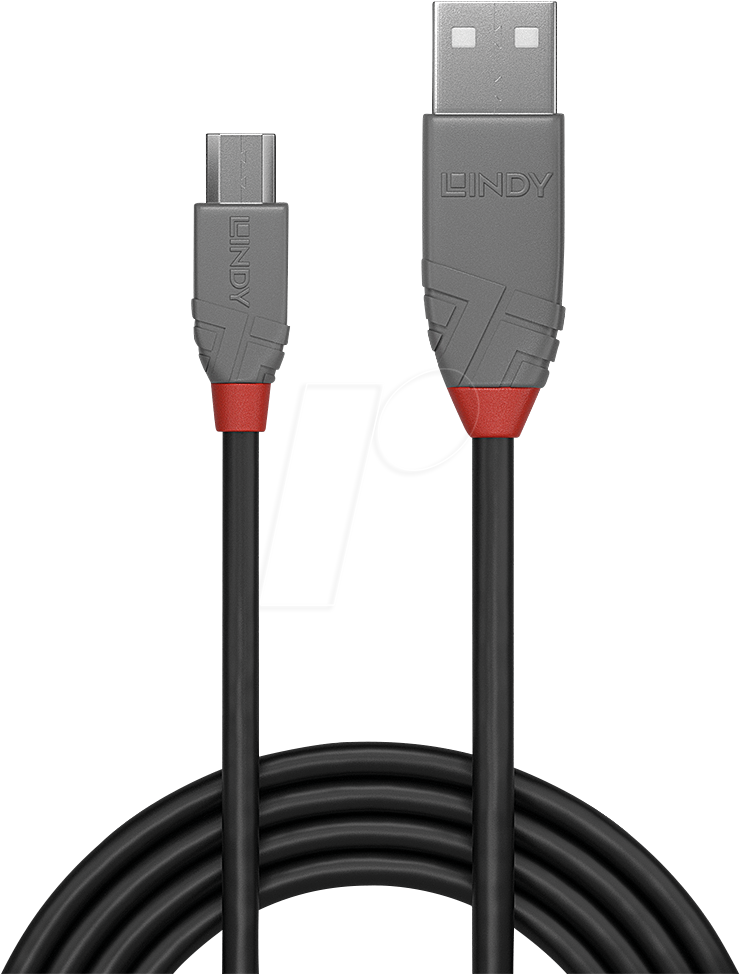
\includegraphics[width=3cm]{Images/BillofMaterials/USB}
	\caption{\textbf{USB}}
	\label{fig:USB}
\end{figure}

\section{Sticky Tape}

\textbf{tesa® WALLPAPER} is a thin but tear-resistant masking tape that has been specially developed for use on very sensitive surfaces such as paper wallpaper or fine plaster. The wallpaper tape is easy to apply, allows precise work with clean paint edges, and can be removed within seven days without leaving any residue. Since the masking tape is suitable for all types of paint, it is the ideal basis for renovation work where you want to protect sensitive surfaces indoors.

\subsection{Features}
\begin{itemize}[noitemsep]
	\item Specially designed for sensitive surfaces such as paper wallpaper.
	\item Masking tape can be removed without leaving any residue for up to seven days.
	\item Solvent-free and primarily made from renewable raw materials.
	\item Suitable for all types of paint.
\end{itemize}

\subsection{Dimensions}
\begin{itemize}[noitemsep]
	\item \textbf{Width:} 25 mm
	\item \textbf{Length:} 25 m
	\item \textbf{Quantity:} 1 Roll
\end{itemize}

\textbf{Metrics}
\begin{itemize}[noitemsep]
	\item \textbf{Length:} 25 m
	\item \textbf{Width:} 25 mm
\end{itemize}

\textbf{Other}
\begin{itemize}[noitemsep]
	\item \textbf{Specification:} For sensitive substrates
\end{itemize}

\textbf{Packaging}
\begin{itemize}[noitemsep]
	\item \textbf{Packaging:} 1 roll
\end{itemize}

\textbf{Manufacturer}
\begin{itemize}[noitemsep]
	\item \textbf{Manufacturer:} TESA
	\item \textbf{Manufacturer's Article Number:} 56260-00000-03
	\item \textbf{Tare:} 0.0787 kg
	\item \textbf{RoHS:} Compliant
	\item \textbf{EAN / GTIN:} 4042448149992
\end{itemize}


\begin{figure}[h!]\centering
	
\includegraphics[width=3cm]{Images/BillofMaterials/Tape}
	\caption{\textbf{Tapes}}
	\label{fig:Tape}
\end{figure}
